\documentclass[dvipdfmx]{jsarticle}
\usepackage[dvipdfmx]{graphicx}
\graphicspath{{ピクチャ/}}
\usepackage{otf}
\usepackage[dvipdfmx]{graphicx}
\usepackage{amsmath,amssymb}
\usepackage{url}
\usepackage{caption}
\begin{document}

\title{\huge 英語論文セミナー 第三回}
\date{}
\maketitle

\begin{flushright}
2022/6/6\\
学籍番号:s0319007\\
氏名:上野智也\\
\end{flushright}

\section{本文}

次に、圧力を変化させた場合の性能について説明する。また、60 kbar までのルビー蛍光スペクトルのシフトに対して光学検出磁気共鳴シフトを較正し、圧力を感知する能力(20)と高圧での光学検出磁気共鳴実験を行う能力を確認した。私たちは、この装置が圧力を変化させても超伝導転移に対する感度を失わないことを示すことを目的とした。図3Aは、7つの圧力点におけるNV$_{\rm C}$のゼーマン分裂の温度依存性を示しており、ここからT$_{\rm C}$の圧力依存性を検出することができる。また、交流磁化率データの裏付けは(20)に記載されている。その結果得られた$T-p$相図(図3B)($p$は圧力)には、圧力とともに超伝導状態が抑制されることが示されている。これは、$x = 0.41$が超伝導ドームのオーバードープ側に位置していることと矛盾しない(25)。また、再現性を検証するために、放出圧力のデータも収集した。$p$に対する$T_{\rm C}$の全体的な滑らかな変化は、この系が弾性領域にあることを示している。この一連の実験により、本技術の性能が確認された。

図2Fの2つの方法の遷移幅は、顕著な違いを示している。これは、磁場をかけることで、第二種超伝導体中で渦糸状態を安定化させることができるからである。光学検出磁気共鳴を用いた手法で幅が大きくなっているのは、試料に近接した窒素空孔が貫通磁場を渦糸という形で感知し始めたためである(試料全体の平均応答を探る交流帯磁率は、渦糸の状態に対する感度が非常に低い)。相境界を探るため、NV$_{\rm C}$で感知した試料C軸に沿った磁場を計算した。8.3 kbar での合成磁場の温度依存性を図 4A に示す。T$_{\rm C1}$以下、T$_{\rm C2}$以上では、C軸磁場は温度非依存である。しかし、T$_{\rm C1}$からT$_{\rm C2}$にかけては、C軸磁場の急激な上昇が検出される。これは、$T > T_{\rm C1}$では磁力線が渦糸の形で入り込み、$T > T_{\rm C2}$では印加した磁力線が完全に入り込んでいることの結果である。常伝導状態である30Kのデータを使って、印加磁場の値を校正することができる。したがって、この磁場は$T_{\rm C1}ではH_{\rm C1}に比例し、T_{\rm C2}ではH_{\rm C2}$に等しいはずである。したがって、我々の光学磁気共鳴データは、圧力下でのマイスナー状態から渦糸状態への遷移を検出する可能性を提供する。

異なる印加磁場での測定を繰り返す、私たちは$\alpha H_{\rm C1}(T)とH_{\rm C2}(T)$を8.3 kbar下$x=0.41$で探し出すことができ(図4B)、$H_{\rm C1}(T)$はマイスナー状態と渦糸状態の境界線である、$\alpha$~0.5は、試料の形状に依存する数値定数である。$H_{\rm c1}(T)$からロンドン侵入長さの温度依存性を導き出し、超伝導ギャップ関数を議論することができる(27, 28)。$H_{\rm c1}(T)$は低温で線形的に現れ、0Kで384Gに外挿される。線形性と外挿された$H_{\rm c1}(0)の値は、この鉄系超伝導体に対してマイクロホール・プローブ・アレイを用いて行われた過去のH_{\rm c1}$研究とよく一致している(27)。一方、初期の傾き$|dH_{\rm C2}
/ dT|_{T_C}$は、自由電子質量に対する準粒子有効質量の二乗に比例する。$H_{C2}(T)$がほぼ垂直であることは、物質系の強相関性と一致する。

我々は、ダイヤモンド中の窒素空孔中心を、極低温条件下の圧力セルにおいて、優れた空間分解能と磁場感度を有するベクトル磁場センサーとして使用することに成功した。ここで示した方法の空間分解能は、100 nm未満に押し上げることができる(20)。この分解能は、圧力セル内の磁区、渦糸(29-32)、スキルミオンなど、磁気関連の特徴のダイナミクスを感知する明確な機会を提供する。非侵襲的かつ非接触の方法であるため、二次元材料の薄片など、従来の巨視的な磁場センサーでは小さすぎたり繊細すぎたりするシステムの研究に用いることができる(33)。さらに、この方法は磁場センシングに限定されるものではない。窒素空孔中心は、局所電場や機械的歪みなど、他の物理パラメータに敏感である。したがって、今回示した方法は、磁場関連プロセス以外にも応用可能であり、圧力下の強相関系における量子物理学の研究において強力なツールとなる。

\begin{figure}[h]
\centering
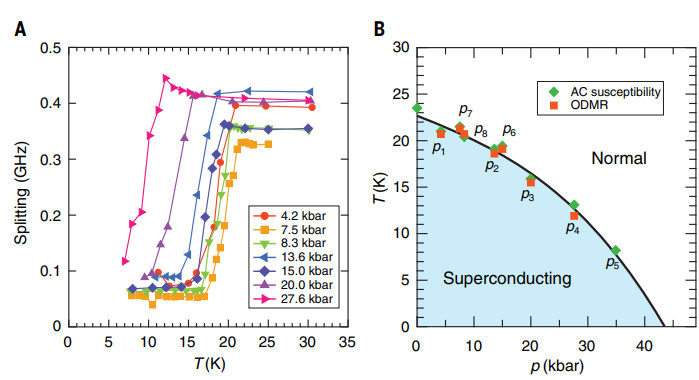
\includegraphics[width=15cm]{fig3.png}
\caption*{図3.窒素空孔センターによるBaFe$_2$(As$_{0.59}$P$_{0.41}$)$_2$温度-圧力相図}
\end{figure}%

・図3のステートメント

(A)異なる圧力下で窒素空孔中心のゼーマン分裂によって測定された超伝導に伴う反磁性。印加磁場は(70$\pm$5)G。

(B)光学磁気共鳴法(緑のひし形)と交流磁化率(赤の四角)で測定した$T_{\rm C}$の、印加圧力に対する変化を示す。$"p1...p8 "$は印加圧力の順序を示す。エラーバーはシンボルサイズより小さくなっている。

\newpage

\begin{figure}[h]
\centering
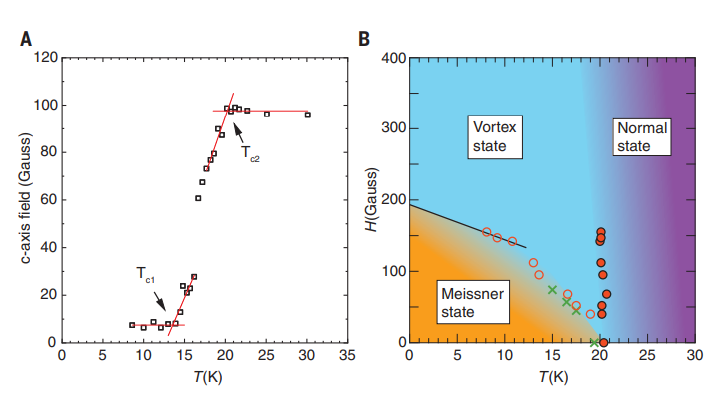
\includegraphics[width=15cm]{fig4.png}
\caption*{図4.BaFe$_2$(As$_{0.59}$P$_{0.41}$)$_2$の下部臨界磁場$H_{\rm C1}(T) と上部臨界磁場 H_{\rm C2}(T)$ の測定。}
\end{figure}%

・図4のステートメント

(A)NV$_{\rm C}$で測定されたc軸方向の磁場。c軸方向の印加電界は95Gであり、これは30Kでのデータから求めることができる。$T_{\rm C1}とT_{\rm C2}$の定義を示す。

(B)8.3kbarでの$\alpha H_{\rm C1}{\rm (T)}(赤色開丸)とH_{\rm_C2}{\rm (T)}$(赤色実線丸)の相図。ここで、磁場に沿った長さ$l_C$と磁場に垂直な長さ$l_a$の薄いスラブのジオメトリ係数$\alpha$は、$\alpha = \tanh(\sqrt{0.36(I_{\rm c}/I_{\rm a})})$ (35) で計算でき、$l_{\rm c}/l_{\rm a} ~ 0.8$である。したがって、$\alpha$は~0.5となる。黒い線は目のガイドの役割を果たす。比較のため、15kbarの$\alpha H_{\rm C1}(T)$を相図に追加した(緑の十字)。エラーバーはシンボルサイズより小さい。

\newpage

\section{用語}

・超伝導ドーム

超伝導体の相図において超伝導を示す部分((25)参照)。

\begin{figure}[h]
\centering
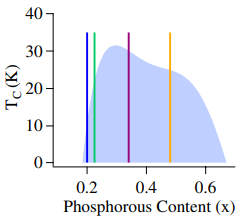
\includegraphics[width=4cm]{SCD.png}
\caption{BaFe$_2$(As$_{0.59}$P$_{0.41}$)$_2$の超伝導ドーム}
\end{figure}%

  

・ロンドン侵入長さ

超伝導状態の超伝導体に入り込む磁場の長さ。

  

・超伝導ギャップ

超伝導体においてフェルミ面付近の電子密度が存在しない、つまりギャップが生じていることを言う。

  

・外挿

ある既知の数値データを基にして、そのデータの範囲の外側で予想される数値を求めること。

  

・マイクロホール・プローブ・アレイ

テーパ形状(先細り)の穴を持つ多層配線基板との接続部品である((27)参照)。

  

・準粒子質量

相互作用をもつ多粒子の集団による運動の中で、振動や波動が量子化され、粒子のように振る舞うため、粒子のように扱うことができるもののことである(例:フォノン(格子振動の量子化)、マグノン(スピン波の量子化))。

  

・磁区

強磁性体中にいくつかの領域があり、その領域内では磁化の方向がそろっている。この領域を磁区という。

  

・スキルミオン

磁性体のスピンや液晶の配向秩序といったベクトル的に表現される秩序を考えると、空間的に一様な秩序の中の局所的な領域において、その一様な秩序とは異なる状態へと連続的に変化しているような構造が、スキルミオンである(多くの場合は、渦状の構造をとる)。





\end{document}